\documentclass[1p]{elsarticle_modified}
%\bibliographystyle{elsarticle-num}

%\usepackage[colorlinks]{hyperref}
%\usepackage{abbrmath_seonhwa} %\Abb, \Ascr, \Acal ,\Abf, \Afrak
\usepackage{amsfonts}
\usepackage{amssymb}
\usepackage{amsmath}
\usepackage{amsthm}
\usepackage{scalefnt}
\usepackage{amsbsy}
\usepackage{kotex}
\usepackage{caption}
\usepackage{subfig}
\usepackage{color}
\usepackage{graphicx}
\usepackage{xcolor} %% white, black, red, green, blue, cyan, magenta, yellow
\usepackage{float}
\usepackage{setspace}
\usepackage{hyperref}

\usepackage{tikz}
\usetikzlibrary{arrows}

\usepackage{multirow}
\usepackage{array} % fixed length table
\usepackage{hhline}

%%%%%%%%%%%%%%%%%%%%%
\makeatletter
\renewcommand*\env@matrix[1][\arraystretch]{%
	\edef\arraystretch{#1}%
	\hskip -\arraycolsep
	\let\@ifnextchar\new@ifnextchar
	\array{*\c@MaxMatrixCols c}}
\makeatother %https://tex.stackexchange.com/questions/14071/how-can-i-increase-the-line-spacing-in-a-matrix
%%%%%%%%%%%%%%%

\usepackage[normalem]{ulem}

\newcommand{\msout}[1]{\ifmmode\text{\sout{\ensuremath{#1}}}\else\sout{#1}\fi}
%SOURCE: \msout is \stkout macro in https://tex.stackexchange.com/questions/20609/strikeout-in-math-mode

\newcommand{\cancel}[1]{
	\ifmmode
	{\color{red}\msout{#1}}
	\else
	{\color{red}\sout{#1}}
	\fi
}

\newcommand{\add}[1]{
	{\color{blue}\uwave{#1}}
}

\newcommand{\replace}[2]{
	\ifmmode
	{\color{red}\msout{#1}}{\color{blue}\uwave{#2}}
	\else
	{\color{red}\sout{#1}}{\color{blue}\uwave{#2}}
	\fi
}

\newcommand{\Sol}{\mathcal{S}} %segment
\newcommand{\D}{D} %diagram
\newcommand{\A}{\mathcal{A}} %arc


%%%%%%%%%%%%%%%%%%%%%%%%%%%%%5 test

\def\sl{\operatorname{\textup{SL}}(2,\Cbb)}
\def\psl{\operatorname{\textup{PSL}}(2,\Cbb)}
\def\quan{\mkern 1mu \triangleright \mkern 1mu}

\theoremstyle{definition}
\newtheorem{thm}{Theorem}[section]
\newtheorem{prop}[thm]{Proposition}
\newtheorem{lem}[thm]{Lemma}
\newtheorem{ques}[thm]{Question}
\newtheorem{cor}[thm]{Corollary}
\newtheorem{defn}[thm]{Definition}
\newtheorem{exam}[thm]{Example}
\newtheorem{rmk}[thm]{Remark}
\newtheorem{alg}[thm]{Algorithm}

\newcommand{\I}{\sqrt{-1}}
\begin{document}

%\begin{frontmatter}
%
%\title{Boundary parabolic representations of knots up to 8 crossings}
%
%%% Group authors per affiliation:
%\author{Yunhi Cho} 
%\address{Department of Mathematics, University of Seoul, Seoul, Korea}
%\ead{yhcho@uos.ac.kr}
%
%
%\author{Seonhwa Kim} %\fnref{s_kim}}
%\address{Center for Geometry and Physics, Institute for Basic Science, Pohang, 37673, Korea}
%\ead{ryeona17@ibs.re.kr}
%
%\author{Hyuk Kim}
%\address{Department of Mathematical Sciences, Seoul National University, Seoul 08826, Korea}
%\ead{hyukkim@snu.ac.kr}
%
%\author{Seokbeom Yoon}
%\address{Department of Mathematical Sciences, Seoul National University, Seoul, 08826,  Korea}
%\ead{sbyoon15@snu.ac.kr}
%
%\begin{abstract}
%We find all boundary parabolic representation of knots up to 8 crossings.
%
%\end{abstract}
%\begin{keyword}
%    \MSC[2010] 57M25 
%\end{keyword}
%
%\end{frontmatter}

%\linenumbers
%\tableofcontents
%
\newcommand\colored[1]{\textcolor{white}{\rule[-0.35ex]{0.8em}{1.4ex}}\kern-0.8em\color{red} #1}%
%\newcommand\colored[1]{\textcolor{white}{ #1}\kern-2.17ex	\textcolor{white}{ #1}\kern-1.81ex	\textcolor{white}{ #1}\kern-2.15ex\color{red}#1	}

{\Large $\underline{12n_{0824}~(K12n_{0824})}$}

\setlength{\tabcolsep}{10pt}
\renewcommand{\arraystretch}{1.6}
\vspace{1cm}\begin{tabular}{m{100pt}>{\centering\arraybackslash}m{274pt}}
\multirow{5}{120pt}{
	\centering
	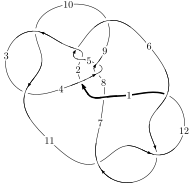
\includegraphics[width=112pt]{../../../GIT/diagram.site/Diagrams/png/2913_12n_0824.png}\\
\ \ \ A knot diagram\footnotemark}&
\allowdisplaybreaks
\textbf{Linearized knot diagam} \\
\cline{2-2}
 &
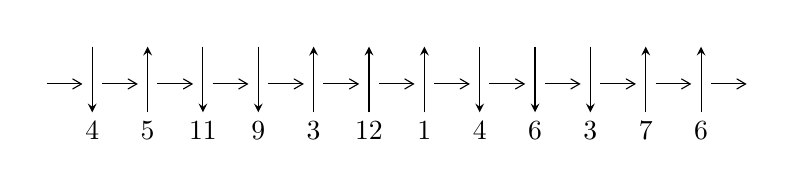
\begin{tikzpicture}[x=20pt, y=17pt]
	% nodes
	\node (C0) at (0, 0) {};
	\node (C1) at (1, 0) {};
	\node (C1U) at (1, +1) {};
	\node (C1D) at (1, -1) {4};

	\node (C2) at (2, 0) {};
	\node (C2U) at (2, +1) {};
	\node (C2D) at (2, -1) {5};

	\node (C3) at (3, 0) {};
	\node (C3U) at (3, +1) {};
	\node (C3D) at (3, -1) {11};

	\node (C4) at (4, 0) {};
	\node (C4U) at (4, +1) {};
	\node (C4D) at (4, -1) {9};

	\node (C5) at (5, 0) {};
	\node (C5U) at (5, +1) {};
	\node (C5D) at (5, -1) {3};

	\node (C6) at (6, 0) {};
	\node (C6U) at (6, +1) {};
	\node (C6D) at (6, -1) {12};

	\node (C7) at (7, 0) {};
	\node (C7U) at (7, +1) {};
	\node (C7D) at (7, -1) {1};

	\node (C8) at (8, 0) {};
	\node (C8U) at (8, +1) {};
	\node (C8D) at (8, -1) {4};

	\node (C9) at (9, 0) {};
	\node (C9U) at (9, +1) {};
	\node (C9D) at (9, -1) {6};

	\node (C10) at (10, 0) {};
	\node (C10U) at (10, +1) {};
	\node (C10D) at (10, -1) {3};

	\node (C11) at (11, 0) {};
	\node (C11U) at (11, +1) {};
	\node (C11D) at (11, -1) {7};

	\node (C12) at (12, 0) {};
	\node (C12U) at (12, +1) {};
	\node (C12D) at (12, -1) {6};
	\node (C13) at (13, 0) {};

	% arrows
	\draw[->,>={angle 60}]
	(C0) edge (C1) (C1) edge (C2) (C2) edge (C3) (C3) edge (C4) (C4) edge (C5) (C5) edge (C6) (C6) edge (C7) (C7) edge (C8) (C8) edge (C9) (C9) edge (C10) (C10) edge (C11) (C11) edge (C12) (C12) edge (C13) ;	\draw[->,>=stealth]
	(C1U) edge (C1D) (C2D) edge (C2U) (C3U) edge (C3D) (C4U) edge (C4D) (C5D) edge (C5U) (C6D) edge (C6U) (C7D) edge (C7U) (C8U) edge (C8D) (C9U) edge (C9D) (C10U) edge (C10D) (C11D) edge (C11U) (C12D) edge (C12U) ;
	\end{tikzpicture} \\
\hhline{~~} \\& 
\textbf{Solving Sequence} \\ \cline{2-2} 
 &
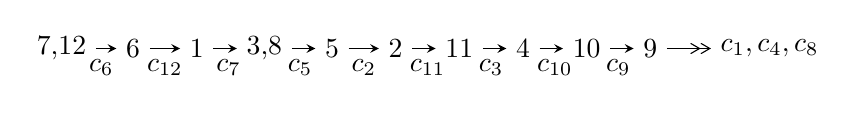
\begin{tikzpicture}[x=23pt, y=7pt]
	% node
	\node (A0) at (-1/8, 0) {7,12};
	\node (A1) at (1, 0) {6};
	\node (A2) at (2, 0) {1};
	\node (A3) at (49/16, 0) {3,8};
	\node (A4) at (33/8, 0) {5};
	\node (A5) at (41/8, 0) {2};
	\node (A6) at (49/8, 0) {11};
	\node (A7) at (57/8, 0) {4};
	\node (A8) at (65/8, 0) {10};
	\node (A9) at (73/8, 0) {9};
	\node (C1) at (1/2, -1) {$c_{6}$};
	\node (C2) at (3/2, -1) {$c_{12}$};
	\node (C3) at (5/2, -1) {$c_{7}$};
	\node (C4) at (29/8, -1) {$c_{5}$};
	\node (C5) at (37/8, -1) {$c_{2}$};
	\node (C6) at (45/8, -1) {$c_{11}$};
	\node (C7) at (53/8, -1) {$c_{3}$};
	\node (C8) at (61/8, -1) {$c_{10}$};
	\node (C9) at (69/8, -1) {$c_{9}$};
	\node (A10) at (11, 0) {$c_{1},c_{4},c_{8}$};

	% edge
	\draw[->,>=stealth]	
	(A0) edge (A1) (A1) edge (A2) (A2) edge (A3) (A3) edge (A4) (A4) edge (A5) (A5) edge (A6) (A6) edge (A7) (A7) edge (A8) (A8) edge (A9) ;
	\draw[->>,>={angle 60}]	
	(A9) edge (A10);
\end{tikzpicture} \\ 

\end{tabular} \\

\footnotetext{
The image of knot diagram is generated by the software ``\textbf{Draw programme}" developed by Andrew Bartholomew(\url{http://www.layer8.co.uk/maths/draw/index.htm\#Running-draw}), where we modified some parts for our purpose(\url{https://github.com/CATsTAILs/LinksPainter}).
}\phantom \\ \newline 
\centering \textbf{Ideals for irreducible components\footnotemark of $X_{\text{par}}$} 
 
\begin{align*}
I^u_{1}&=\langle 
u^{19}-4 u^{18}+\cdots+2 b-16,\;u^{19}-3 u^{18}+\cdots+2 a+7,\;u^{20}-4 u^{19}+\cdots-10 u+4\rangle \\
I^u_{2}&=\langle 
u^{11}+2 u^{10}+5 u^9+7 u^8+7 u^7+7 u^6+u^5-2 u^4-3 u^3-4 u^2+b+1,\\
\phantom{I^u_{2}}&\phantom{= \langle  }-2 u^{11}-3 u^{10}-11 u^9-13 u^8-21 u^7-20 u^6-14 u^5-8 u^4+2 u^3+6 u^2+a+4 u+3,\\
\phantom{I^u_{2}}&\phantom{= \langle  }u^{12}+u^{11}+6 u^{10}+5 u^9+13 u^8+9 u^7+10 u^6+5 u^5-2 u^4-3 u^3-4 u^2-3 u+1\rangle \\
I^u_{3}&=\langle 
-309 u^5 a^3+1269 u^5 a^2+\cdots+3300 a-2645,\;- u^5 a^2+5 u^5 a+\cdots+20 a-22,\\
\phantom{I^u_{3}}&\phantom{= \langle  }u^6+u^5+3 u^4+2 u^3+2 u^2+u-1\rangle \\
\\
\end{align*}
\raggedright * 3 irreducible components of $\dim_{\mathbb{C}}=0$, with total 56 representations.\\
\footnotetext{All coefficients of polynomials are rational numbers. But the coefficients are sometimes approximated in decimal forms when there is not enough margin.}
\newpage
\renewcommand{\arraystretch}{1}
\centering \section*{I. $I^u_{1}= \langle u^{19}-4 u^{18}+\cdots+2 b-16,\;u^{19}-3 u^{18}+\cdots+2 a+7,\;u^{20}-4 u^{19}+\cdots-10 u+4 \rangle$}
\flushleft \textbf{(i) Arc colorings}\\
\begin{tabular}{m{7pt} m{180pt} m{7pt} m{180pt} }
\flushright $a_{7}=$&$\begin{pmatrix}1\\0\end{pmatrix}$ \\
\flushright $a_{12}=$&$\begin{pmatrix}0\\u\end{pmatrix}$ \\
\flushright $a_{6}=$&$\begin{pmatrix}1\\u^2\end{pmatrix}$ \\
\flushright $a_{1}=$&$\begin{pmatrix}u\\u^3+u\end{pmatrix}$ \\
\flushright $a_{3}=$&$\begin{pmatrix}-\frac{1}{2} u^{19}+\frac{3}{2} u^{18}+\cdots+\frac{9}{2} u-\frac{7}{2}\\-\frac{1}{2} u^{19}+2 u^{18}+\cdots-\frac{17}{2} u+8\end{pmatrix}$ \\
\flushright $a_{8}=$&$\begin{pmatrix}- u^4- u^2+1\\- u^6-2 u^4- u^2\end{pmatrix}$ \\
\flushright $a_{5}=$&$\begin{pmatrix}\frac{1}{4} u^{19}-\frac{1}{2} u^{18}+\cdots-\frac{9}{4} u+3\\\frac{1}{2} u^{19}-2 u^{18}+\cdots+\frac{11}{2} u-5\end{pmatrix}$ \\
\flushright $a_{2}=$&$\begin{pmatrix}-\frac{1}{4} u^{19}+\frac{1}{2} u^{18}+\cdots-\frac{7}{4} u+3\\-\frac{1}{2} u^{19}+2 u^{18}+\cdots-\frac{3}{2} u-1\end{pmatrix}$ \\
\flushright $a_{11}=$&$\begin{pmatrix}- u\\u\end{pmatrix}$ \\
\flushright $a_{4}=$&$\begin{pmatrix}-\frac{1}{2} u^{19}+\frac{3}{2} u^{18}+\cdots+\frac{11}{2} u-\frac{11}{2}\\-\frac{1}{2} u^{19}+2 u^{18}+\cdots-\frac{19}{2} u+10\end{pmatrix}$ \\
\flushright $a_{10}=$&$\begin{pmatrix}-\frac{3}{4} u^{19}+\frac{5}{2} u^{18}+\cdots-\frac{21}{4} u+3\\\frac{1}{2} u^{19}-2 u^{18}+\cdots+\frac{7}{2} u-1\end{pmatrix}$ \\
\flushright $a_{9}=$&$\begin{pmatrix}-\frac{1}{4} u^{19}+\frac{1}{2} u^{18}+\cdots-2 u^2+\frac{1}{4} u\\\frac{1}{2} u^{19}- u^{18}+\cdots+\frac{3}{2} u-1\end{pmatrix}$\\&\end{tabular}
\flushleft \textbf{(ii) Obstruction class $= -1$}\\~\\
\flushleft \textbf{(iii) Cusp Shapes $= -7 u^{19}+18 u^{18}-80 u^{17}+154 u^{16}-358 u^{15}+536 u^{14}-813 u^{13}+973 u^{12}-1035 u^{11}+1062 u^{10}-910 u^9+941 u^8-875 u^7+831 u^6-754 u^5+461 u^4-286 u^3+94 u^2-10 u+26$}\\~\\
\newpage\renewcommand{\arraystretch}{1}
\flushleft \textbf{(iv) u-Polynomials at the component}\newline \\
\begin{tabular}{m{50pt}|m{274pt}}
Crossings & \hspace{64pt}u-Polynomials at each crossing \\
\hline $$\begin{aligned}c_{1}\end{aligned}$$&$\begin{aligned}
&u^{20}-3 u^{19}+\cdots+u+1
\end{aligned}$\\
\hline $$\begin{aligned}c_{2},c_{5}\end{aligned}$$&$\begin{aligned}
&u^{20}+10 u^{19}+\cdots+96 u+64
\end{aligned}$\\
\hline $$\begin{aligned}c_{3},c_{4},c_{8}\\c_{10}\end{aligned}$$&$\begin{aligned}
&u^{20}- u^{19}+\cdots+u+1
\end{aligned}$\\
\hline $$\begin{aligned}c_{6},c_{11},c_{12}\end{aligned}$$&$\begin{aligned}
&u^{20}+4 u^{19}+\cdots+10 u+4
\end{aligned}$\\
\hline $$\begin{aligned}c_{7}\end{aligned}$$&$\begin{aligned}
&u^{20}-4 u^{19}+\cdots-702 u+180
\end{aligned}$\\
\hline $$\begin{aligned}c_{9}\end{aligned}$$&$\begin{aligned}
&u^{20}+u^{19}+\cdots+u+1
\end{aligned}$\\
\hline
\end{tabular}\\~\\
\newpage\renewcommand{\arraystretch}{1}
\flushleft \textbf{(v) Riley Polynomials at the component}\newline \\
\begin{tabular}{m{50pt}|m{274pt}}
Crossings & \hspace{64pt}Riley Polynomials at each crossing \\
\hline $$\begin{aligned}c_{1}\end{aligned}$$&$\begin{aligned}
&y^{20}+37 y^{19}+\cdots+39 y+1
\end{aligned}$\\
\hline $$\begin{aligned}c_{2},c_{5}\end{aligned}$$&$\begin{aligned}
&y^{20}-18 y^{19}+\cdots+15360 y+4096
\end{aligned}$\\
\hline $$\begin{aligned}c_{3},c_{4},c_{8}\\c_{10}\end{aligned}$$&$\begin{aligned}
&y^{20}+5 y^{19}+\cdots+7 y+1
\end{aligned}$\\
\hline $$\begin{aligned}c_{6},c_{11},c_{12}\end{aligned}$$&$\begin{aligned}
&y^{20}+16 y^{19}+\cdots+84 y+16
\end{aligned}$\\
\hline $$\begin{aligned}c_{7}\end{aligned}$$&$\begin{aligned}
&y^{20}-16 y^{19}+\cdots+203796 y+32400
\end{aligned}$\\
\hline $$\begin{aligned}c_{9}\end{aligned}$$&$\begin{aligned}
&y^{20}+45 y^{19}+\cdots+47 y+1
\end{aligned}$\\
\hline
\end{tabular}\\~\\
\newpage\flushleft \textbf{(vi) Complex Volumes and Cusp Shapes}
$$\begin{array}{c|c|c}  
\text{Solutions to }I^u_{1}& \I (\text{vol} + \sqrt{-1}CS) & \text{Cusp shape}\\
 \hline 
\begin{aligned}
u &= -0.803867 + 0.553658 I \\
a &= -0.349654 - 0.706335 I \\
b &= \phantom{-}0.551090 - 0.058137 I\end{aligned}
 & \phantom{-}4.62986 - 2.72937 I & \phantom{-}8.70348 + 10.27722 I \\ \hline\begin{aligned}
u &= -0.803867 - 0.553658 I \\
a &= -0.349654 + 0.706335 I \\
b &= \phantom{-}0.551090 + 0.058137 I\end{aligned}
 & \phantom{-}4.62986 + 2.72937 I & \phantom{-}8.70348 - 10.27722 I \\ \hline\begin{aligned}
u &= \phantom{-}0.918506 + 0.116805 I \\
a &= -1.36529 + 0.79203 I \\
b &= \phantom{-}0.368555 + 0.693111 I\end{aligned}
 & \phantom{-}12.0452 + 8.8841 I & \phantom{-}3.76642 - 4.75992 I \\ \hline\begin{aligned}
u &= \phantom{-}0.918506 - 0.116805 I \\
a &= -1.36529 - 0.79203 I \\
b &= \phantom{-}0.368555 - 0.693111 I\end{aligned}
 & \phantom{-}12.0452 - 8.8841 I & \phantom{-}3.76642 + 4.75992 I \\ \hline\begin{aligned}
u &= \phantom{-}0.324780 + 1.157920 I \\
a &= -0.864339 + 0.054005 I \\
b &= \phantom{-}0.1230180 + 0.0513018 I\end{aligned}
 & \phantom{-}0.778843 + 0.268408 I & \phantom{-}0.81841 + 2.57430 I \\ \hline\begin{aligned}
u &= \phantom{-}0.324780 - 1.157920 I \\
a &= -0.864339 - 0.054005 I \\
b &= \phantom{-}0.1230180 - 0.0513018 I\end{aligned}
 & \phantom{-}0.778843 - 0.268408 I & \phantom{-}0.81841 - 2.57430 I \\ \hline\begin{aligned}
u &= \phantom{-}0.790212 + 0.106147 I \\
a &= \phantom{-}0.786114 - 0.120277 I \\
b &= -0.311017 - 0.987779 I\end{aligned}
 & \phantom{-}3.96682 + 3.79390 I & \phantom{-}4.34323 - 7.18597 I \\ \hline\begin{aligned}
u &= \phantom{-}0.790212 - 0.106147 I \\
a &= \phantom{-}0.786114 + 0.120277 I \\
b &= -0.311017 + 0.987779 I\end{aligned}
 & \phantom{-}3.96682 - 3.79390 I & \phantom{-}4.34323 + 7.18597 I \\ \hline\begin{aligned}
u &= \phantom{-}0.497474 + 1.173310 I \\
a &= \phantom{-}0.040811 + 0.371019 I \\
b &= \phantom{-}1.152440 - 0.664354 I\end{aligned}
 & \phantom{-}8.80911 - 3.86307 I & \phantom{-}1.37632 + 1.51742 I \\ \hline\begin{aligned}
u &= \phantom{-}0.497474 - 1.173310 I \\
a &= \phantom{-}0.040811 - 0.371019 I \\
b &= \phantom{-}1.152440 + 0.664354 I\end{aligned}
 & \phantom{-}8.80911 + 3.86307 I & \phantom{-}1.37632 - 1.51742 I\\
 \hline 
 \end{array}$$\newpage$$\begin{array}{c|c|c}  
\text{Solutions to }I^u_{1}& \I (\text{vol} + \sqrt{-1}CS) & \text{Cusp shape}\\
 \hline 
\begin{aligned}
u &= -0.034804 + 1.372190 I \\
a &= -0.01189 + 1.58136 I \\
b &= \phantom{-}0.28579 - 2.05494 I\end{aligned}
 & -5.57112 - 1.57630 I & -4.91455 + 4.16839 I \\ \hline\begin{aligned}
u &= -0.034804 - 1.372190 I \\
a &= -0.01189 - 1.58136 I \\
b &= \phantom{-}0.28579 + 2.05494 I\end{aligned}
 & -5.57112 + 1.57630 I & -4.91455 - 4.16839 I \\ \hline\begin{aligned}
u &= \phantom{-}0.341712 + 1.335550 I \\
a &= \phantom{-}0.64325 - 1.79998 I \\
b &= -0.16720 + 2.35614 I\end{aligned}
 & -0.56408 + 7.88066 I & -0.02470 - 9.49068 I \\ \hline\begin{aligned}
u &= \phantom{-}0.341712 - 1.335550 I \\
a &= \phantom{-}0.64325 + 1.79998 I \\
b &= -0.16720 - 2.35614 I\end{aligned}
 & -0.56408 - 7.88066 I & -0.02470 + 9.49068 I \\ \hline\begin{aligned}
u &= \phantom{-}0.41375 + 1.36143 I \\
a &= -0.02752 + 2.02004 I \\
b &= -0.53548 - 3.06612 I\end{aligned}
 & \phantom{-}7.4013 + 13.6532 I & -0.15677 - 6.88804 I \\ \hline\begin{aligned}
u &= \phantom{-}0.41375 - 1.36143 I \\
a &= -0.02752 - 2.02004 I \\
b &= -0.53548 + 3.06612 I\end{aligned}
 & \phantom{-}7.4013 - 13.6532 I & -0.15677 + 6.88804 I \\ \hline\begin{aligned}
u &= -0.23877 + 1.45754 I \\
a &= \phantom{-}0.61208 - 1.29474 I \\
b &= -0.89507 + 1.82927 I\end{aligned}
 & -1.86609 - 6.35619 I & -4.51758 + 8.10478 I \\ \hline\begin{aligned}
u &= -0.23877 - 1.45754 I \\
a &= \phantom{-}0.61208 + 1.29474 I \\
b &= -0.89507 - 1.82927 I\end{aligned}
 & -1.86609 + 6.35619 I & -4.51758 - 8.10478 I \\ \hline\begin{aligned}
u &= -0.208998 + 0.404596 I \\
a &= -0.463566 + 0.573101 I \\
b &= -0.072115 + 0.396543 I\end{aligned}
 & -0.021058 - 0.934804 I & -0.39426 + 7.39454 I \\ \hline\begin{aligned}
u &= -0.208998 - 0.404596 I \\
a &= -0.463566 - 0.573101 I \\
b &= -0.072115 - 0.396543 I\end{aligned}
 & -0.021058 + 0.934804 I & -0.39426 - 7.39454 I\\
 \hline 
 \end{array}$$\newpage\newpage\renewcommand{\arraystretch}{1}
\centering \section*{II. $I^u_{2}= \langle u^{11}+2 u^{10}+\cdots+b+1,\;-2 u^{11}-3 u^{10}+\cdots+a+3,\;u^{12}+u^{11}+\cdots-3 u+1 \rangle$}
\flushleft \textbf{(i) Arc colorings}\\
\begin{tabular}{m{7pt} m{180pt} m{7pt} m{180pt} }
\flushright $a_{7}=$&$\begin{pmatrix}1\\0\end{pmatrix}$ \\
\flushright $a_{12}=$&$\begin{pmatrix}0\\u\end{pmatrix}$ \\
\flushright $a_{6}=$&$\begin{pmatrix}1\\u^2\end{pmatrix}$ \\
\flushright $a_{1}=$&$\begin{pmatrix}u\\u^3+u\end{pmatrix}$ \\
\flushright $a_{3}=$&$\begin{pmatrix}2 u^{11}+3 u^{10}+\cdots-4 u-3\\- u^{11}-2 u^{10}-5 u^9-7 u^8-7 u^7-7 u^6- u^5+2 u^4+3 u^3+4 u^2-1\end{pmatrix}$ \\
\flushright $a_{8}=$&$\begin{pmatrix}- u^4- u^2+1\\- u^6-2 u^4- u^2\end{pmatrix}$ \\
\flushright $a_{5}=$&$\begin{pmatrix}- u^9-4 u^7- u^6-6 u^5-4 u^4-2 u^3-3 u^2+u+3\\- u^8- u^7-3 u^6-2 u^5- u^4- u^3+3 u^2+u\end{pmatrix}$ \\
\flushright $a_{2}=$&$\begin{pmatrix}- u^{11}- u^{10}-4 u^9-4 u^8-4 u^7-4 u^6+3 u^5+3 u^4+4 u^3+5 u^2- u-3\\u^{11}+u^{10}+5 u^9+5 u^8+9 u^7+8 u^6+5 u^5+2 u^4- u^3-5 u^2- u\end{pmatrix}$ \\
\flushright $a_{11}=$&$\begin{pmatrix}- u\\u\end{pmatrix}$ \\
\flushright $a_{4}=$&$\begin{pmatrix}2 u^{11}+2 u^{10}+\cdots-3 u-3\\- u^{11}- u^{10}-4 u^9-3 u^8-4 u^7-2 u^6+2 u^5+3 u^4+3 u^3+3 u^2- u-1\end{pmatrix}$ \\
\flushright $a_{10}=$&$\begin{pmatrix}- u^9- u^8-5 u^7-4 u^6-8 u^5-5 u^4-2 u^3+u^2+4 u+4\\- u^{11}-2 u^{10}-6 u^9-9 u^8-12 u^7-13 u^6-7 u^5-2 u^4+4 u^3+6 u^2+3 u\end{pmatrix}$ \\
\flushright $a_{9}=$&$\begin{pmatrix}- u^{10}-2 u^9-6 u^8-9 u^7-12 u^6-13 u^5-8 u^4-2 u^3+3 u^2+7 u+4\\- u^{11}- u^{10}-5 u^9-4 u^8-8 u^7-6 u^6-2 u^5-2 u^4+4 u^3+2 u^2+1\end{pmatrix}$\\&\end{tabular}
\flushleft \textbf{(ii) Obstruction class $= 1$}\\~\\
\flushleft \textbf{(iii) Cusp Shapes $= 8 u^{11}+7 u^{10}+39 u^9+28 u^8+67 u^7+41 u^6+35 u^5+17 u^4-12 u^3-11 u^2-9 u-9$}\\~\\
\newpage\renewcommand{\arraystretch}{1}
\flushleft \textbf{(iv) u-Polynomials at the component}\newline \\
\begin{tabular}{m{50pt}|m{274pt}}
Crossings & \hspace{64pt}u-Polynomials at each crossing \\
\hline $$\begin{aligned}c_{1}\end{aligned}$$&$\begin{aligned}
&u^{12}+3 u^{11}+\cdots-3 u-1
\end{aligned}$\\
\hline $$\begin{aligned}c_{2}\end{aligned}$$&$\begin{aligned}
&u^{12}+3 u^{11}+\cdots-7 u+3
\end{aligned}$\\
\hline $$\begin{aligned}c_{3},c_{8}\end{aligned}$$&$\begin{aligned}
&u^{12}+u^{11}-4 u^{10}-4 u^9+3 u^8+4 u^7+4 u^6+u^5-3 u^4-2 u^3-2 u^2- u-1
\end{aligned}$\\
\hline $$\begin{aligned}c_{4},c_{10}\end{aligned}$$&$\begin{aligned}
&u^{12}- u^{11}-4 u^{10}+4 u^9+3 u^8-4 u^7+4 u^6- u^5-3 u^4+2 u^3-2 u^2+u-1
\end{aligned}$\\
\hline $$\begin{aligned}c_{5}\end{aligned}$$&$\begin{aligned}
&u^{12}-3 u^{11}+\cdots+7 u+3
\end{aligned}$\\
\hline $$\begin{aligned}c_{6}\end{aligned}$$&$\begin{aligned}
&u^{12}+u^{11}+\cdots-3 u+1
\end{aligned}$\\
\hline $$\begin{aligned}c_{7}\end{aligned}$$&$\begin{aligned}
&u^{12}- u^{11}+\cdots-5 u+1
\end{aligned}$\\
\hline $$\begin{aligned}c_{9}\end{aligned}$$&$\begin{aligned}
&u^{12}+u^{11}+2 u^{10}+2 u^9+3 u^8- u^7-4 u^6-4 u^5-3 u^4+4 u^3+4 u^2- u-1
\end{aligned}$\\
\hline $$\begin{aligned}c_{11},c_{12}\end{aligned}$$&$\begin{aligned}
&u^{12}- u^{11}+\cdots+3 u+1
\end{aligned}$\\
\hline
\end{tabular}\\~\\
\newpage\renewcommand{\arraystretch}{1}
\flushleft \textbf{(v) Riley Polynomials at the component}\newline \\
\begin{tabular}{m{50pt}|m{274pt}}
Crossings & \hspace{64pt}Riley Polynomials at each crossing \\
\hline $$\begin{aligned}c_{1}\end{aligned}$$&$\begin{aligned}
&y^{12}-5 y^{11}+\cdots-5 y+1
\end{aligned}$\\
\hline $$\begin{aligned}c_{2},c_{5}\end{aligned}$$&$\begin{aligned}
&y^{12}-15 y^{11}+\cdots-79 y+9
\end{aligned}$\\
\hline $$\begin{aligned}c_{3},c_{4},c_{8}\\c_{10}\end{aligned}$$&$\begin{aligned}
&y^{12}-9 y^{11}+\cdots+3 y+1
\end{aligned}$\\
\hline $$\begin{aligned}c_{6},c_{11},c_{12}\end{aligned}$$&$\begin{aligned}
&y^{12}+11 y^{11}+\cdots-17 y+1
\end{aligned}$\\
\hline $$\begin{aligned}c_{7}\end{aligned}$$&$\begin{aligned}
&y^{12}-9 y^{11}+\cdots-19 y+1
\end{aligned}$\\
\hline $$\begin{aligned}c_{9}\end{aligned}$$&$\begin{aligned}
&y^{12}+3 y^{11}+\cdots-9 y+1
\end{aligned}$\\
\hline
\end{tabular}\\~\\
\newpage\flushleft \textbf{(vi) Complex Volumes and Cusp Shapes}
$$\begin{array}{c|c|c}  
\text{Solutions to }I^u_{2}& \I (\text{vol} + \sqrt{-1}CS) & \text{Cusp shape}\\
 \hline 
\begin{aligned}
u &= -0.779914 + 0.263433 I \\
a &= -0.739356 - 0.514285 I \\
b &= \phantom{-}0.685921 - 0.270227 I\end{aligned}
 & \phantom{-}4.49844 - 1.95126 I & \phantom{-}6.47342 + 1.58269 I \\ \hline\begin{aligned}
u &= -0.779914 - 0.263433 I \\
a &= -0.739356 + 0.514285 I \\
b &= \phantom{-}0.685921 + 0.270227 I\end{aligned}
 & \phantom{-}4.49844 + 1.95126 I & \phantom{-}6.47342 - 1.58269 I \\ \hline\begin{aligned}
u &= -0.207510 + 1.165490 I \\
a &= \phantom{-}1.28081 - 1.18072 I \\
b &= -0.553497 + 1.171330 I\end{aligned}
 & \phantom{-}2.05176 - 1.39702 I & \phantom{-}4.75145 + 0.05437 I \\ \hline\begin{aligned}
u &= -0.207510 - 1.165490 I \\
a &= \phantom{-}1.28081 + 1.18072 I \\
b &= -0.553497 - 1.171330 I\end{aligned}
 & \phantom{-}2.05176 + 1.39702 I & \phantom{-}4.75145 - 0.05437 I \\ \hline\begin{aligned}
u &= \phantom{-}0.725402\phantom{ +0.000000I} \\
a &= \phantom{-}2.12667\phantom{ +0.000000I} \\
b &= -0.0816291\phantom{ +0.000000I}\end{aligned}
 & -1.30199\phantom{ +0.000000I} & \phantom{-}3.72770\phantom{ +0.000000I} \\ \hline\begin{aligned}
u &= \phantom{-}0.074423 + 1.296140 I \\
a &= -1.09122 + 1.86397 I \\
b &= \phantom{-}0.98699 - 2.82215 I\end{aligned}
 & -7.89835 + 1.11402 I & -9.81262 + 0.65462 I \\ \hline\begin{aligned}
u &= \phantom{-}0.074423 - 1.296140 I \\
a &= -1.09122 - 1.86397 I \\
b &= \phantom{-}0.98699 + 2.82215 I\end{aligned}
 & -7.89835 - 1.11402 I & -9.81262 - 0.65462 I \\ \hline\begin{aligned}
u &= \phantom{-}0.298860 + 1.278450 I \\
a &= \phantom{-}0.58549 - 1.60488 I \\
b &= -0.90103 + 2.69883 I\end{aligned}
 & -5.28054 + 3.69650 I & -1.82268 - 3.88848 I \\ \hline\begin{aligned}
u &= \phantom{-}0.298860 - 1.278450 I \\
a &= \phantom{-}0.58549 + 1.60488 I \\
b &= -0.90103 - 2.69883 I\end{aligned}
 & -5.28054 - 3.69650 I & -1.82268 + 3.88848 I \\ \hline\begin{aligned}
u &= -0.36930 + 1.39020 I \\
a &= \phantom{-}0.050962 - 1.233380 I \\
b &= -0.31739 + 1.65322 I\end{aligned}
 & -0.69950 - 6.22445 I & \phantom{-}1.48925 + 7.33691 I\\
 \hline 
 \end{array}$$\newpage$$\begin{array}{c|c|c}  
\text{Solutions to }I^u_{2}& \I (\text{vol} + \sqrt{-1}CS) & \text{Cusp shape}\\
 \hline 
\begin{aligned}
u &= -0.36930 - 1.39020 I \\
a &= \phantom{-}0.050962 + 1.233380 I \\
b &= -0.31739 - 1.65322 I\end{aligned}
 & -0.69950 + 6.22445 I & \phantom{-}1.48925 - 7.33691 I \\ \hline\begin{aligned}
u &= \phantom{-}0.241471\phantom{ +0.000000I} \\
a &= -4.30005\phantom{ +0.000000I} \\
b &= -0.720367\phantom{ +0.000000I}\end{aligned}
 & -3.78082\phantom{ +0.000000I} & -11.8850\phantom{ +0.000000I}\\
 \hline 
 \end{array}$$\newpage\newpage\renewcommand{\arraystretch}{1}
\centering \section*{III. $I^u_{3}= \langle -309 u^5 a^3+1269 u^5 a^2+\cdots+3300 a-2645,\;- u^5 a^2+5 u^5 a+\cdots+20 a-22,\;u^6+u^5+3 u^4+2 u^3+2 u^2+u-1 \rangle$}
\flushleft \textbf{(i) Arc colorings}\\
\begin{tabular}{m{7pt} m{180pt} m{7pt} m{180pt} }
\flushright $a_{7}=$&$\begin{pmatrix}1\\0\end{pmatrix}$ \\
\flushright $a_{12}=$&$\begin{pmatrix}0\\u\end{pmatrix}$ \\
\flushright $a_{6}=$&$\begin{pmatrix}1\\u^2\end{pmatrix}$ \\
\flushright $a_{1}=$&$\begin{pmatrix}u\\u^3+u\end{pmatrix}$ \\
\flushright $a_{3}=$&$\begin{pmatrix}a\\0.121797 a^{3} u^{5}-0.500197 a^{2} u^{5}+\cdots-1.30075 a+1.04257\end{pmatrix}$ \\
\flushright $a_{8}=$&$\begin{pmatrix}- u^4- u^2+1\\u^5+u^4+2 u^3+u^2+u-1\end{pmatrix}$ \\
\flushright $a_{5}=$&$\begin{pmatrix}0.164762 a^{3} u^{5}+0.0555775 a^{2} u^{5}+\cdots-1.46788 a+3.80922\\-0.338195 a^{3} u^{5}+0.146630 a^{2} u^{5}+\cdots+1.05952 a-0.137170\end{pmatrix}$ \\
\flushright $a_{2}=$&$\begin{pmatrix}0.0429641 a^{3} u^{5}+0.555775 a^{2} u^{5}+\cdots-0.167127 a+1.76665\\0.272369 a^{3} u^{5}-0.547103 a^{2} u^{5}+\cdots+0.214032 a-0.430430\end{pmatrix}$ \\
\flushright $a_{11}=$&$\begin{pmatrix}- u\\u\end{pmatrix}$ \\
\flushright $a_{4}=$&$\begin{pmatrix}0.610564 a^{3} u^{5}-0.693733 a^{2} u^{5}+\cdots+0.154513 a-0.293260\\-0.488766 a^{3} u^{5}+0.193536 a^{2} u^{5}+\cdots-0.455262 a+1.33583\end{pmatrix}$ \\
\flushright $a_{10}=$&$\begin{pmatrix}-0.00827749 a^{3} u^{5}+0.296807 a^{2} u^{5}+\cdots-0.118644 a+1.19196\\0.144265 a^{3} u^{5}-0.368940 a^{2} u^{5}+\cdots-1.35081 a+1.45842\end{pmatrix}$ \\
\flushright $a_{9}=$&$\begin{pmatrix}-0.140323 a^{3} u^{5}-0.357115 a^{2} u^{5}+\cdots-0.864013 a+2.53212\\-0.00827749 a^{3} u^{5}+0.296807 a^{2} u^{5}+\cdots-0.118644 a+1.19196\end{pmatrix}$\\&\end{tabular}
\flushleft \textbf{(ii) Obstruction class $= -1$}\\~\\
\flushleft \textbf{(iii) Cusp Shapes $= 4 u^4+4 u^3+8 u^2+4 u+2$}\\~\\
\newpage\renewcommand{\arraystretch}{1}
\flushleft \textbf{(iv) u-Polynomials at the component}\newline \\
\begin{tabular}{m{50pt}|m{274pt}}
Crossings & \hspace{64pt}u-Polynomials at each crossing \\
\hline $$\begin{aligned}c_{1}\end{aligned}$$&$\begin{aligned}
&u^{24}-5 u^{23}+\cdots+3370 u-89
\end{aligned}$\\
\hline $$\begin{aligned}c_{2},c_{5}\end{aligned}$$&$\begin{aligned}
&(u^2- u-1)^{12}
\end{aligned}$\\
\hline $$\begin{aligned}c_{3},c_{4},c_{8}\\c_{10}\end{aligned}$$&$\begin{aligned}
&u^{24}- u^{23}+\cdots-64 u-31
\end{aligned}$\\
\hline $$\begin{aligned}c_{6},c_{11},c_{12}\end{aligned}$$&$\begin{aligned}
&(u^6- u^5+3 u^4-2 u^3+2 u^2- u-1)^4
\end{aligned}$\\
\hline $$\begin{aligned}c_{7}\end{aligned}$$&$\begin{aligned}
&(u^6+u^5-3 u^4-2 u^3+2 u^2- u-1)^4
\end{aligned}$\\
\hline $$\begin{aligned}c_{9}\end{aligned}$$&$\begin{aligned}
&u^{24}+u^{23}+\cdots+244 u-509
\end{aligned}$\\
\hline
\end{tabular}\\~\\
\newpage\renewcommand{\arraystretch}{1}
\flushleft \textbf{(v) Riley Polynomials at the component}\newline \\
\begin{tabular}{m{50pt}|m{274pt}}
Crossings & \hspace{64pt}Riley Polynomials at each crossing \\
\hline $$\begin{aligned}c_{1}\end{aligned}$$&$\begin{aligned}
&y^{24}+7 y^{23}+\cdots-10179964 y+7921
\end{aligned}$\\
\hline $$\begin{aligned}c_{2},c_{5}\end{aligned}$$&$\begin{aligned}
&(y^2-3 y+1)^{12}
\end{aligned}$\\
\hline $$\begin{aligned}c_{3},c_{4},c_{8}\\c_{10}\end{aligned}$$&$\begin{aligned}
&y^{24}-5 y^{23}+\cdots+120 y+961
\end{aligned}$\\
\hline $$\begin{aligned}c_{6},c_{11},c_{12}\end{aligned}$$&$\begin{aligned}
&(y^6+5 y^5+9 y^4+4 y^3-6 y^2-5 y+1)^4
\end{aligned}$\\
\hline $$\begin{aligned}c_{7}\end{aligned}$$&$\begin{aligned}
&(y^6-7 y^5+17 y^4-16 y^3+6 y^2-5 y+1)^4
\end{aligned}$\\
\hline $$\begin{aligned}c_{9}\end{aligned}$$&$\begin{aligned}
&y^{24}+19 y^{23}+\cdots-1812532 y+259081
\end{aligned}$\\
\hline
\end{tabular}\\~\\
\newpage\flushleft \textbf{(vi) Complex Volumes and Cusp Shapes}
$$\begin{array}{c|c|c}  
\text{Solutions to }I^u_{3}& \I (\text{vol} + \sqrt{-1}CS) & \text{Cusp shape}\\
 \hline 
\begin{aligned}
u &= -0.873214\phantom{ +0.000000I} \\
a &= -0.659674 + 0.470538 I \\
b &= \phantom{-}0.115030 + 0.358787 I\end{aligned}
 & \phantom{-}3.71224\phantom{ +0.000000I} & \phantom{-}4.26950\phantom{ +0.000000I} \\ \hline\begin{aligned}
u &= -0.873214\phantom{ +0.000000I} \\
a &= -0.659674 - 0.470538 I \\
b &= \phantom{-}0.115030 - 0.358787 I\end{aligned}
 & \phantom{-}3.71224\phantom{ +0.000000I} & \phantom{-}4.26950\phantom{ +0.000000I} \\ \hline\begin{aligned}
u &= -0.873214\phantom{ +0.000000I} \\
a &= \phantom{-}1.72705 + 0.77873 I \\
b &= -0.301154 + 0.593781 I\end{aligned}
 & \phantom{-}11.6079\phantom{ +0.000000I} & \phantom{-}4.26950\phantom{ +0.000000I} \\ \hline\begin{aligned}
u &= -0.873214\phantom{ +0.000000I} \\
a &= \phantom{-}1.72705 - 0.77873 I \\
b &= -0.301154 - 0.593781 I\end{aligned}
 & \phantom{-}11.6079\phantom{ +0.000000I} & \phantom{-}4.26950\phantom{ +0.000000I} \\ \hline\begin{aligned}
u &= \phantom{-}0.138835 + 1.234450 I \\
a &= -0.715076 - 0.696779 I \\
b &= -0.303312 + 0.803256 I\end{aligned}
 & \phantom{-}0.98760 + 1.97241 I & -3.42428 - 3.68478 I \\ \hline\begin{aligned}
u &= \phantom{-}0.138835 + 1.234450 I \\
a &= \phantom{-}1.46538 - 0.91785 I \\
b &= -1.27213 + 1.88327 I\end{aligned}
 & -6.90809 + 1.97241 I & -3.42428 - 3.68478 I \\ \hline\begin{aligned}
u &= \phantom{-}0.138835 + 1.234450 I \\
a &= -0.40722 + 2.05651 I \\
b &= \phantom{-}0.52582 - 3.23377 I\end{aligned}
 & -6.90809 + 1.97241 I & -3.42428 - 3.68478 I \\ \hline\begin{aligned}
u &= \phantom{-}0.138835 + 1.234450 I \\
a &= -2.05522 - 2.28427 I \\
b &= \phantom{-}2.25718 + 2.73240 I\end{aligned}
 & \phantom{-}0.98760 + 1.97241 I & -3.42428 - 3.68478 I \\ \hline\begin{aligned}
u &= \phantom{-}0.138835 - 1.234450 I \\
a &= -0.715076 + 0.696779 I \\
b &= -0.303312 - 0.803256 I\end{aligned}
 & \phantom{-}0.98760 - 1.97241 I & -3.42428 + 3.68478 I \\ \hline\begin{aligned}
u &= \phantom{-}0.138835 - 1.234450 I \\
a &= \phantom{-}1.46538 + 0.91785 I \\
b &= -1.27213 - 1.88327 I\end{aligned}
 & -6.90809 - 1.97241 I & -3.42428 + 3.68478 I\\
 \hline 
 \end{array}$$\newpage$$\begin{array}{c|c|c}  
\text{Solutions to }I^u_{3}& \I (\text{vol} + \sqrt{-1}CS) & \text{Cusp shape}\\
 \hline 
\begin{aligned}
u &= \phantom{-}0.138835 - 1.234450 I \\
a &= -0.40722 - 2.05651 I \\
b &= \phantom{-}0.52582 + 3.23377 I\end{aligned}
 & -6.90809 - 1.97241 I & -3.42428 + 3.68478 I \\ \hline\begin{aligned}
u &= \phantom{-}0.138835 - 1.234450 I \\
a &= -2.05522 + 2.28427 I \\
b &= \phantom{-}2.25718 - 2.73240 I\end{aligned}
 & \phantom{-}0.98760 - 1.97241 I & -3.42428 + 3.68478 I \\ \hline\begin{aligned}
u &= -0.408802 + 1.276380 I \\
a &= -0.236388 - 0.995320 I \\
b &= -0.07505 + 1.70186 I\end{aligned}
 & -0.25226 - 4.59213 I & \phantom{-}0.58114 + 3.20482 I \\ \hline\begin{aligned}
u &= -0.408802 + 1.276380 I \\
a &= \phantom{-}0.271082 + 0.518597 I \\
b &= -1.47317 - 1.04109 I\end{aligned}
 & \phantom{-}7.64342 - 4.59213 I & \phantom{-}0.58114 + 3.20482 I \\ \hline\begin{aligned}
u &= -0.408802 + 1.276380 I \\
a &= \phantom{-}0.0568064 + 0.0049770 I \\
b &= \phantom{-}0.540176 - 0.066558 I\end{aligned}
 & -0.25226 - 4.59213 I & \phantom{-}0.58114 + 3.20482 I \\ \hline\begin{aligned}
u &= -0.408802 + 1.276380 I \\
a &= \phantom{-}0.19907 + 2.07416 I \\
b &= \phantom{-}0.25546 - 3.24019 I\end{aligned}
 & \phantom{-}7.64342 - 4.59213 I & \phantom{-}0.58114 + 3.20482 I \\ \hline\begin{aligned}
u &= -0.408802 - 1.276380 I \\
a &= -0.236388 + 0.995320 I \\
b &= -0.07505 - 1.70186 I\end{aligned}
 & -0.25226 + 4.59213 I & \phantom{-}0.58114 - 3.20482 I \\ \hline\begin{aligned}
u &= -0.408802 - 1.276380 I \\
a &= \phantom{-}0.271082 - 0.518597 I \\
b &= -1.47317 + 1.04109 I\end{aligned}
 & \phantom{-}7.64342 + 4.59213 I & \phantom{-}0.58114 - 3.20482 I \\ \hline\begin{aligned}
u &= -0.408802 - 1.276380 I \\
a &= \phantom{-}0.0568064 - 0.0049770 I \\
b &= \phantom{-}0.540176 + 0.066558 I\end{aligned}
 & -0.25226 + 4.59213 I & \phantom{-}0.58114 - 3.20482 I \\ \hline\begin{aligned}
u &= -0.408802 - 1.276380 I \\
a &= \phantom{-}0.19907 - 2.07416 I \\
b &= \phantom{-}0.25546 + 3.24019 I\end{aligned}
 & \phantom{-}7.64342 + 4.59213 I & \phantom{-}0.58114 - 3.20482 I\\
 \hline 
 \end{array}$$\newpage$$\begin{array}{c|c|c}  
\text{Solutions to }I^u_{3}& \I (\text{vol} + \sqrt{-1}CS) & \text{Cusp shape}\\
 \hline 
\begin{aligned}
u &= \phantom{-}0.413150\phantom{ +0.000000I} \\
a &= \phantom{-}1.61499\phantom{ +0.000000I} \\
b &= \phantom{-}0.893703\phantom{ +0.000000I}\end{aligned}
 & -3.20899\phantom{ +0.000000I} & \phantom{-}5.41680\phantom{ +0.000000I} \\ \hline\begin{aligned}
u &= \phantom{-}0.413150\phantom{ +0.000000I} \\
a &= \phantom{-}2.19113 + 1.72840 I \\
b &= -1.244020 + 0.295025 I\end{aligned}
 & \phantom{-}4.68669\phantom{ +0.000000I} & \phantom{-}5.41680\phantom{ +0.000000I} \\ \hline\begin{aligned}
u &= \phantom{-}0.413150\phantom{ +0.000000I} \\
a &= \phantom{-}2.19113 - 1.72840 I \\
b &= -1.244020 - 0.295025 I\end{aligned}
 & \phantom{-}4.68669\phantom{ +0.000000I} & \phantom{-}5.41680\phantom{ +0.000000I} \\ \hline\begin{aligned}
u &= \phantom{-}0.413150\phantom{ +0.000000I} \\
a &= -3.28887\phantom{ +0.000000I} \\
b &= \phantom{-}0.0566461\phantom{ +0.000000I}\end{aligned}
 & -3.20899\phantom{ +0.000000I} & \phantom{-}5.41680\phantom{ +0.000000I}\\
 \hline 
 \end{array}$$\newpage
\newpage\renewcommand{\arraystretch}{1}
\centering \section*{ IV. u-Polynomials}
\begin{tabular}{m{50pt}|m{274pt}}
Crossings & \hspace{64pt}u-Polynomials at each crossing \\
\hline $$\begin{aligned}c_{1}\end{aligned}$$&$\begin{aligned}
&(u^{12}+3 u^{11}+\cdots-3 u-1)(u^{20}-3 u^{19}+\cdots+u+1)\\
&\cdot(u^{24}-5 u^{23}+\cdots+3370 u-89)
\end{aligned}$\\
\hline $$\begin{aligned}c_{2}\end{aligned}$$&$\begin{aligned}
&((u^2- u-1)^{12})(u^{12}+3 u^{11}+\cdots-7 u+3)(u^{20}+10 u^{19}+\cdots+96 u+64)
\end{aligned}$\\
\hline $$\begin{aligned}c_{3},c_{8}\end{aligned}$$&$\begin{aligned}
&(u^{12}+u^{11}-4 u^{10}-4 u^9+3 u^8+4 u^7+4 u^6+u^5-3 u^4-2 u^3-2 u^2- u-1)\\
&\cdot(u^{20}- u^{19}+\cdots+u+1)(u^{24}- u^{23}+\cdots-64 u-31)
\end{aligned}$\\
\hline $$\begin{aligned}c_{4},c_{10}\end{aligned}$$&$\begin{aligned}
&(u^{12}- u^{11}-4 u^{10}+4 u^9+3 u^8-4 u^7+4 u^6- u^5-3 u^4+2 u^3-2 u^2+u-1)\\
&\cdot(u^{20}- u^{19}+\cdots+u+1)(u^{24}- u^{23}+\cdots-64 u-31)
\end{aligned}$\\
\hline $$\begin{aligned}c_{5}\end{aligned}$$&$\begin{aligned}
&((u^2- u-1)^{12})(u^{12}-3 u^{11}+\cdots+7 u+3)(u^{20}+10 u^{19}+\cdots+96 u+64)
\end{aligned}$\\
\hline $$\begin{aligned}c_{6}\end{aligned}$$&$\begin{aligned}
&((u^6- u^5+3 u^4-2 u^3+2 u^2- u-1)^{4})(u^{12}+u^{11}+\cdots-3 u+1)\\
&\cdot(u^{20}+4 u^{19}+\cdots+10 u+4)
\end{aligned}$\\
\hline $$\begin{aligned}c_{7}\end{aligned}$$&$\begin{aligned}
&((u^6+u^5-3 u^4-2 u^3+2 u^2- u-1)^{4})(u^{12}- u^{11}+\cdots-5 u+1)\\
&\cdot(u^{20}-4 u^{19}+\cdots-702 u+180)
\end{aligned}$\\
\hline $$\begin{aligned}c_{9}\end{aligned}$$&$\begin{aligned}
&(u^{12}+u^{11}+2 u^{10}+2 u^9+3 u^8- u^7-4 u^6-4 u^5-3 u^4+4 u^3+4 u^2- u-1)\\
&\cdot(u^{20}+u^{19}+\cdots+u+1)(u^{24}+u^{23}+\cdots+244 u-509)
\end{aligned}$\\
\hline $$\begin{aligned}c_{11},c_{12}\end{aligned}$$&$\begin{aligned}
&((u^6- u^5+3 u^4-2 u^3+2 u^2- u-1)^{4})(u^{12}- u^{11}+\cdots+3 u+1)\\
&\cdot(u^{20}+4 u^{19}+\cdots+10 u+4)
\end{aligned}$\\
\hline
\end{tabular}\newpage\renewcommand{\arraystretch}{1}
\centering \section*{ V. Riley Polynomials}
\begin{tabular}{m{50pt}|m{274pt}}
Crossings & \hspace{64pt}Riley Polynomials at each crossing \\
\hline $$\begin{aligned}c_{1}\end{aligned}$$&$\begin{aligned}
&(y^{12}-5 y^{11}+\cdots-5 y+1)(y^{20}+37 y^{19}+\cdots+39 y+1)\\
&\cdot(y^{24}+7 y^{23}+\cdots-10179964 y+7921)
\end{aligned}$\\
\hline $$\begin{aligned}c_{2},c_{5}\end{aligned}$$&$\begin{aligned}
&((y^2-3 y+1)^{12})(y^{12}-15 y^{11}+\cdots-79 y+9)\\
&\cdot(y^{20}-18 y^{19}+\cdots+15360 y+4096)
\end{aligned}$\\
\hline $$\begin{aligned}c_{3},c_{4},c_{8}\\c_{10}\end{aligned}$$&$\begin{aligned}
&(y^{12}-9 y^{11}+\cdots+3 y+1)(y^{20}+5 y^{19}+\cdots+7 y+1)\\
&\cdot(y^{24}-5 y^{23}+\cdots+120 y+961)
\end{aligned}$\\
\hline $$\begin{aligned}c_{6},c_{11},c_{12}\end{aligned}$$&$\begin{aligned}
&((y^6+5 y^5+\cdots-5 y+1)^{4})(y^{12}+11 y^{11}+\cdots-17 y+1)\\
&\cdot(y^{20}+16 y^{19}+\cdots+84 y+16)
\end{aligned}$\\
\hline $$\begin{aligned}c_{7}\end{aligned}$$&$\begin{aligned}
&((y^6-7 y^5+\cdots-5 y+1)^{4})(y^{12}-9 y^{11}+\cdots-19 y+1)\\
&\cdot(y^{20}-16 y^{19}+\cdots+203796 y+32400)
\end{aligned}$\\
\hline $$\begin{aligned}c_{9}\end{aligned}$$&$\begin{aligned}
&(y^{12}+3 y^{11}+\cdots-9 y+1)(y^{20}+45 y^{19}+\cdots+47 y+1)\\
&\cdot(y^{24}+19 y^{23}+\cdots-1812532 y+259081)
\end{aligned}$\\
\hline
\end{tabular}
\vskip 2pc
\end{document}